In general, results from the microspectrometer are much smoother than results from the fluorimeter, which include quite a lot of noise. \todo{Something about excitation power and noise? Sources?} We suspect that this is a consequence of wide-field illumination used by the fluorimeter, in which molecules outside the region of interest (or otherwise, with some defects) are excited and emit spectra different from that of the region of interest. \note{Maybe not, depending on the power thing.}

\section{ADT TES-F}

For a drop-cast sample of ADT TES-F on glass, we selected a region of interest which appeared to be a single crystal, with few visually distinguishable defects. The crystal was also selected such that its surface area was larger than the area illuminated by the microspectrometer's laser spot. The emission spectra of the region of interest are shown in Figure \ref{fig:pl-adt-tesf}.

\todo{Convert wavelength from nm to eV? This seems to be a more common unit in solid state.}

Both spectra in Figure \ref{fig:pl-adt-tesf} show a clear peak around 630nm, which has been shown in other research.\cite{lam_polarization_2018}\cite{ostroverkhova_organic_2016} The spectra measured by the microspectrometer also shows a secondary peak just below 600 nm, which is not evident in the spectrum taken by the fluorimeter. \todo{Additional sources that back up the peaks I'm showing?}

\begin{figure}[h]
    \centering
    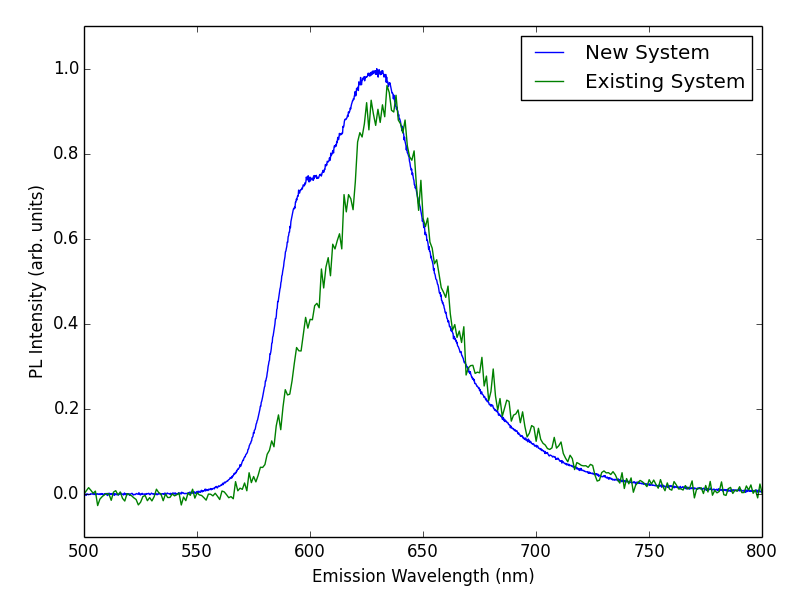
\includegraphics[width=.8\textwidth]{./img/tesf-2.png}%\llap{\raisebox{4cm}{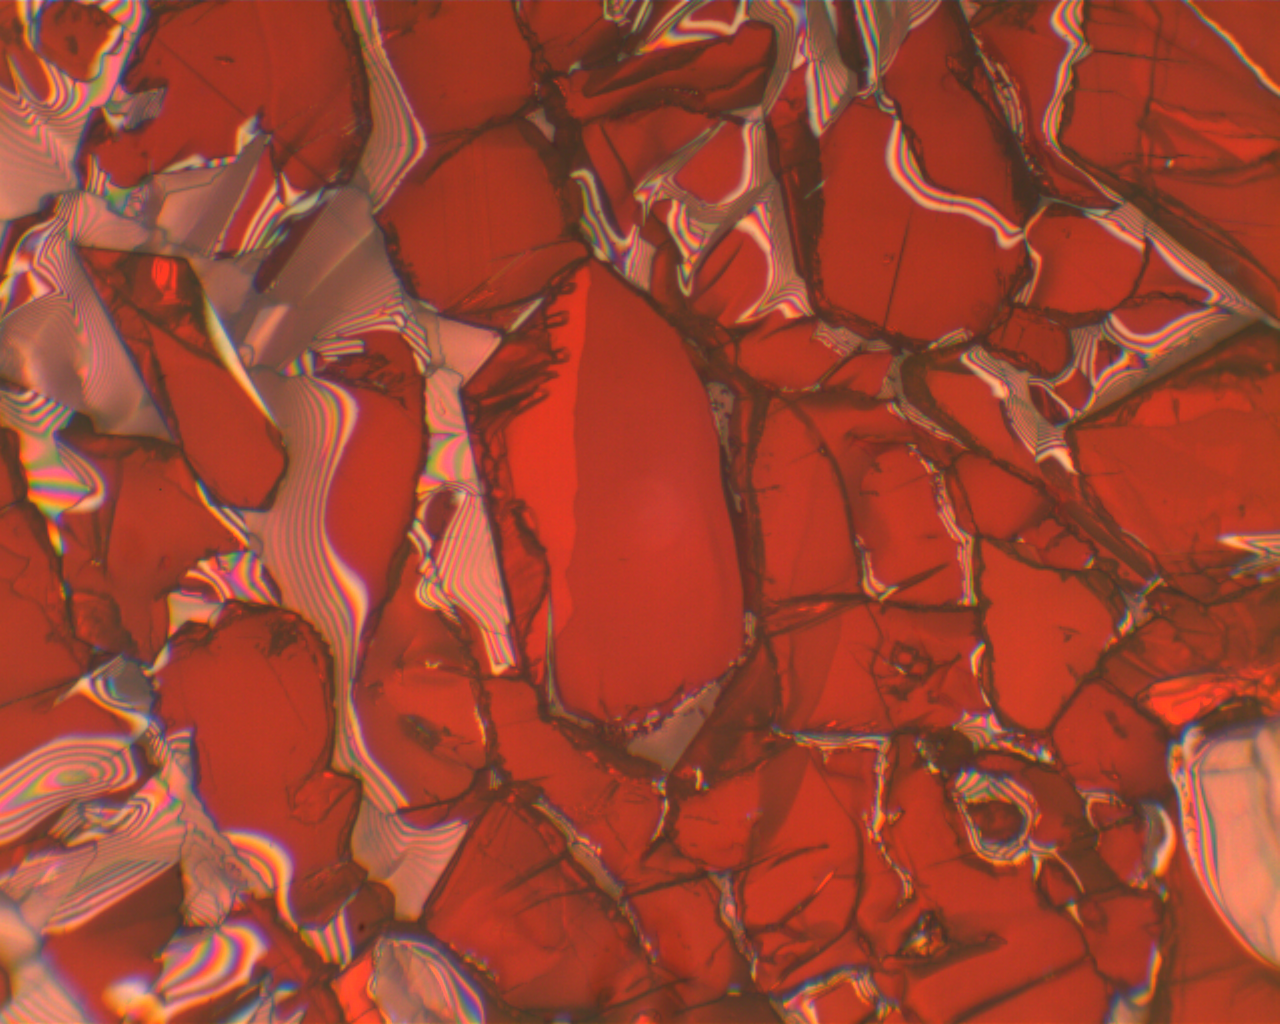
\includegraphics[width=2cm]{img/tesf-white-illum.png}}}
    % 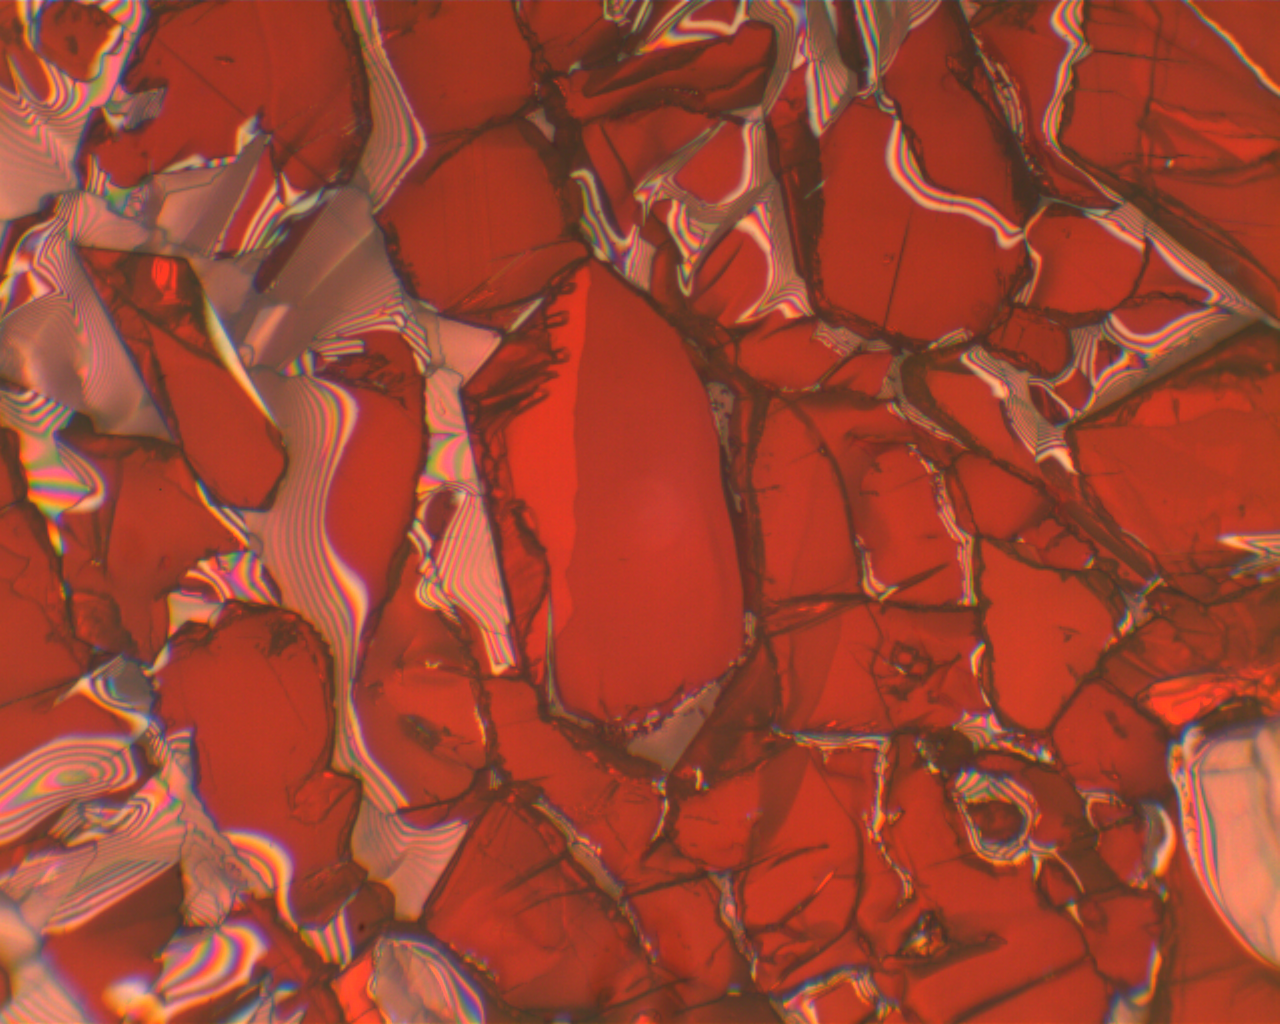
\includegraphics[width=.2\textwidth]{./img/tesf-white-illum.png}
    % 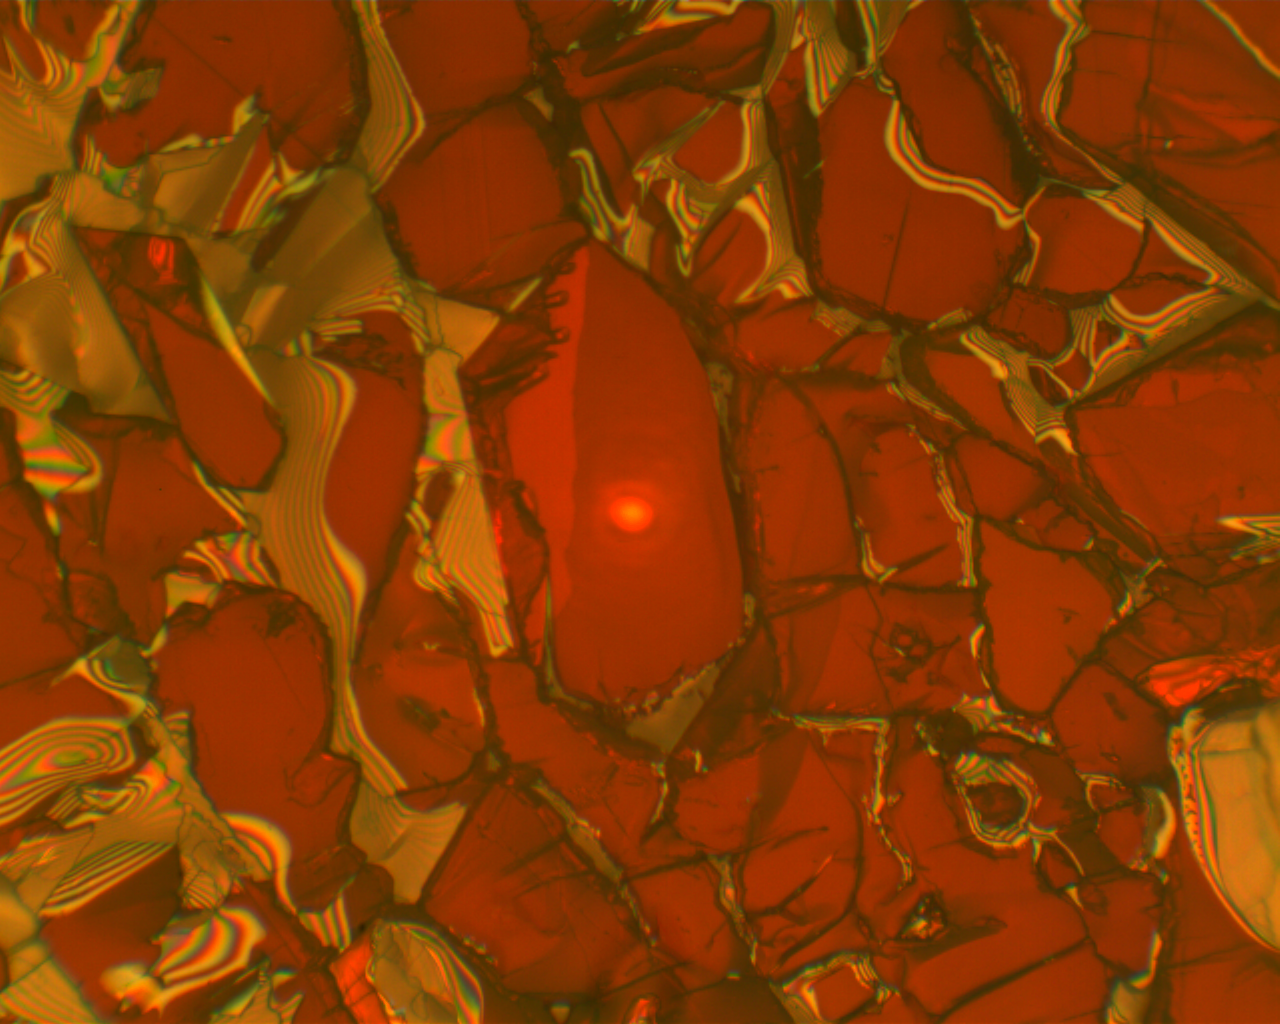
\includegraphics[width=.2\textwidth]{./img/tesf-laser-illum.png}
    \caption[PL emission spectrum of ADT TES-F, excited at 405nm.]{PL emission spectrum of ADT TES-F, excited at 405 nm.
    Wide-field illumination used by the existing system to excite the sample
    yields a noisy spectrum, and does not excite the secondary peak that is 
    shown clearly in the results from the new system. A single crystal, larger than the laser spot, was selected among smaller neighboring crystals for this measurement. %This may be because the
    %wide-field illumination is exciting many adjacent crystals in the sample, 
    %which emit slightly different spectra. The laser illumination in the new 
    %system has the spatial resolution necessary to illuminate single crystals.
    }
    \label{fig:pl-adt-tesf}
\end{figure}

\section{\ce{CdSe} Quantum Dots}
Figure \ref{fig:pl-adt-qd} shows the PL emission of CdSe quantum dots \todo{in solution? on substrate?}. There is one broad, clear peak that aligns well with the same measurement taken on the fluorimeter, between 520 and 620 nm. This peak seems to agree with other studies of CdSe quantum structures.\cite{empedocles_photoluminescence_1996}

Unlike the same measurement taken on ADT, this measurement was taken in a region of interest which is sparsely populated with quantum dots, with one target grouping illuminated by the laser.

\todo{What else do I write about here? Need to find more resources on analysis of PL, i.e. what information we get about the material. This will also be useful for Background section.}

\begin{figure}[h]
    \centering
    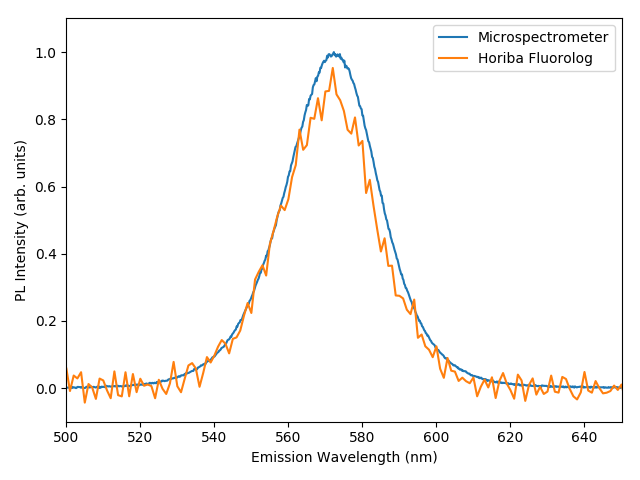
\includegraphics[width=\textwidth]{./img/qd-2.png}
    % 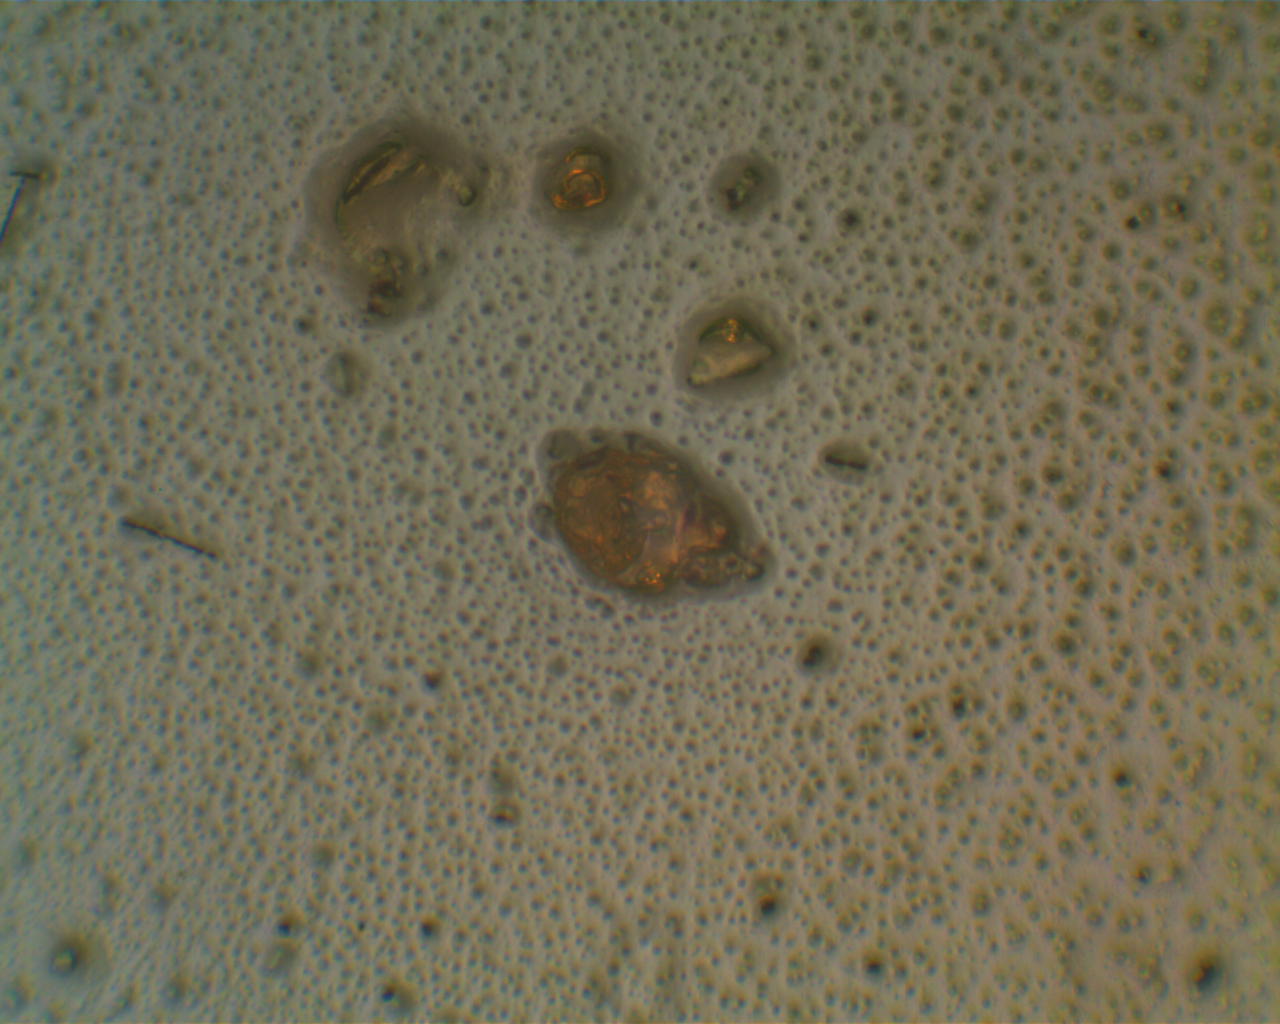
\includegraphics[width=4cm]{./img/qd-white-illum.png}
    % 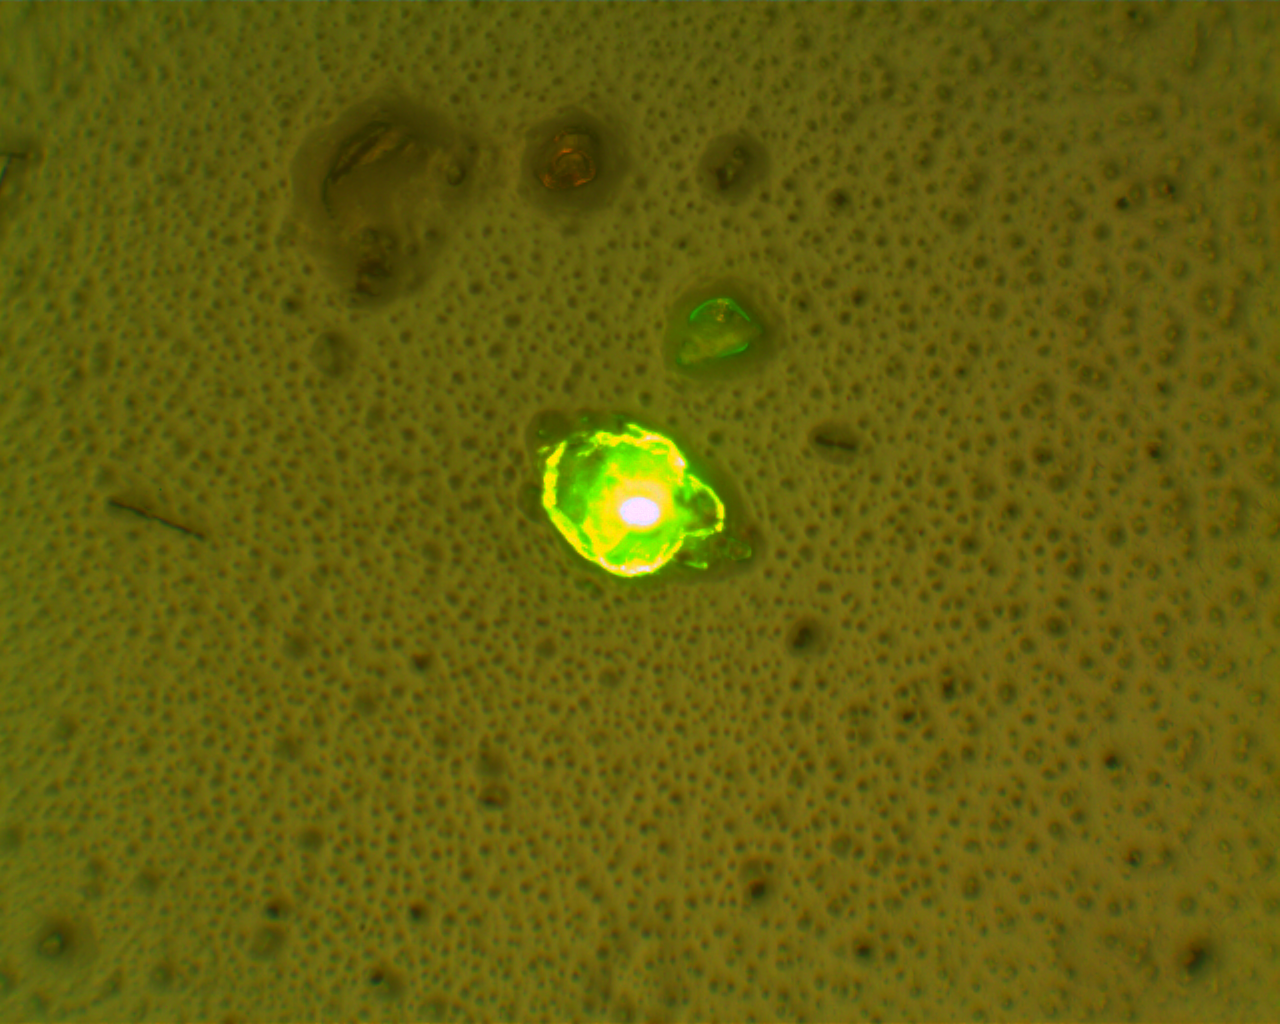
\includegraphics[width=4cm]{./img/qd-laser-illum.png}
    \caption{PL emission spectrum of a cluster of CdSe quantum dots on ?? substrate, excited at 405 nm.}
    \label{fig:pl-adt-qd}
\end{figure}
